\documentclass[a4paper,12pt]{article}
\usepackage[utf8]{inputenc}
\usepackage[german]{babel}
\usepackage{amsmath}
\usepackage{amssymb}
\usepackage{amsthm}
\usepackage{geometry}
\usepackage{graphicx}
\usepackage[hidelinks]{hyperref}
\usepackage{listings}
\usepackage{xcolor}
\usepackage{enumitem}
\usepackage[expansion=false]{microtype}
\usepackage{booktabs}
\usepackage{caption}

\geometry{margin=2.5cm}
\sloppy
\setlength{\emergencystretch}{3em}

\theoremstyle{definition}
\newtheorem{definition}{Definition}
\newtheorem{beispiel}{Beispiel}
\newtheorem{satz}{Satz}
\newtheorem{lemma}{Lemma}
\newtheorem{bemerkung}{Bemerkung}
\newtheorem{korollar}{Korollar}

\setlist[itemize,1]{label=--}

\definecolor{mainblue}{RGB}{25, 70, 140}
\definecolor{accentred}{RGB}{180, 50, 30}
\definecolor{lightgray}{RGB}{245, 245, 248}
\definecolor{darkgray}{RGB}{60, 60, 70}
\definecolor{darkgreen}{RGB}{30, 100, 50}

\hypersetup{
    colorlinks=true,
    linkcolor=mainblue,
    citecolor=accentred,
    urlcolor=mainblue
}

\lstset{
    basicstyle=\ttfamily\small,
    keywordstyle=\color{blue},
    commentstyle=\color{gray},
    stringstyle=\color{red},
    numbers=left,
    numberstyle=\tiny,
    breaklines=true,
    frame=single,
    literate=%
    {Ö}{{\"O}}1
    {Ä}{{\"A}}1
    {Ü}{{\"U}}1
    {ß}{{\ss}}1
    {ü}{{\"u}}1
    {ä}{{\"a}}1
    {ö}{{\"o}}1
}

\title{Pflichtdokumentation im FPGA-Entwurf:\\
Nichtflüchtige Konfiguration, Deployment-Workflow\\
und formale Dokumentationsanforderungen\\\large
Formale Analyse, Verifikation und Best Practices\\
für \texttt{.bit} und \texttt{.bin} auf dem Basys~3}
\author{Stephan Epp}
\date{25. Juni 2026}

\begin{document}

\maketitle
\tableofcontents
\newpage

% ──────────────────────────────────────────────────────────────
\section{Einführung}

Der Entwurf digitaler Schaltungen für FPGA-Plattformen unterscheidet sich von
klassischer Softwareentwicklung fundamental durch die Notwendigkeit der
\emph{Konfiguration} des programmierbaren Hardwaresubstrats. Ein FPGA
(Field Programmable Gate Array) ist ein rekonfigurierbarer Halbleiter,
dessen Logikfunktion durch einen Bitstrom definiert wird, der in
Konfigurationsspeicher geschrieben wird. Zwei grundlegend verschiedene
Speicherarten stehen dabei zur Verfügung: flüchtiger SRAM-Konfigurationsspeicher
und nichtflüchtiger SPI-Flash-Speicher~\cite{xilinx2019,digilent2023}.

Die Unterscheidung zwischen diesen beiden Deployment-Pfaden — dem
\texttt{.bit}-Format für SRAM und dem \texttt{.bin}-Format für Flash —
hat weitreichende Konsequenzen für den gesamten Entwurfsworkflow,
insbesondere für die Dokumentationspflichten. Diese Arbeit stellt die
These auf und beweist formal:

\begin{quote}
\emph{Die nichtflüchtige Konfiguration eines FPGA mittels SPI-Flash impliziert
zwingend eine vollständige Dokumentationspflicht, die integraler Bestandteil
des Entwurfsworkflows sein muss.}
\end{quote}

\subsection{Motivation}

Ein im SPI-Flash eines FPGA-Boards gespeicherter Bitstrom überdauert
Stromverlust, Systemneustarts und physikalischen Transport. Der FPGA
konfiguriert sich beim Einschalten vollautomatisch aus dem Flash — ohne
externe Werkzeuge, ohne Verbindung zum Entwicklungsrechner. Dies macht
ihn zu einem eigenständigen, autonomen Hardwaregerät.

Genau diese Eigenschaft erzeugt die Dokumentationspflicht: Ein Gerät,
das eigenständig funktioniert, muss \emph{verstehbar, reproduzierbar
und wartbar} sein — auch Jahre nach seiner Erstellung, auch ohne den
ursprünglichen Entwickler. Diese Anforderung ist aus der Automobilelektronik
(ISO~26262), der Medizintechnik (IEC~62304) und der Luft- und Raumfahrt
(DO-178C) bekannt und gilt analog für jeden nichtflüchtigen
FPGA-Entwurf~\cite{iso26262,iec62304}.

\subsection{Ziele der Arbeit}

Diese Arbeit verfolgt vier Ziele:
\begin{itemize}
    \item Formale Definition und Abgrenzung von \texttt{.bit} und \texttt{.bin}
          als Konfigurationsformate mit ihren jeweiligen Eigenschaften.
    \item Formaler Nachweis der Dokumentationspflicht für nichtflüchtige Designs.
    \item Spezifikation eines vollständigen Dokumentationsworkflows als
          Bestandteil des FPGA-Entwurfsprozesses.
    \item Praktische Anwendung auf das Basys~3 (Artix-7) Board mit Vivado~2019.2.
\end{itemize}

\subsection{Ãœberblick}

Abschnitt~\ref{sec:grundlagen} legt Grundlagen zu FPGA-Konfiguration und
Dokumentation fest. Abschnitt~\ref{sec:bitbin} analysiert beide
Konfigurationsformate formal. Abschnitt~\ref{sec:pflicht} beweist die
Dokumentationspflicht. Abschnitt~\ref{sec:workflow} spezifiziert den
vollständigen Workflow. Abschnitt~\ref{sec:basys3} zeigt die praktische
Anwendung. Abschnitt~\ref{sec:ausblick} gibt einen ausführlichen Ausblick.

% ──────────────────────────────────────────────────────────────
\section{Grundlagen}
\label{sec:grundlagen}

\subsection{FPGA-Konfigurationsspeicher}

\begin{definition}[FPGA-Konfiguration]
    Die Konfiguration eines FPGA ist die Abbildung eines Bitstroms $\mathcal{B}$
    auf den Konfigurationsspeicher $\mathcal{C}$ des Bausteins:
    \[
    \kappa: \mathcal{B} \to \mathcal{C}, \quad \kappa(\mathcal{B}) = c \in \mathcal{C}.
    \]
    Der Zustand $c$ bestimmt die logische Funktion $f_c: \{0,1\}^n \to \{0,1\}^m$
    des FPGA vollständig.
\end{definition}

\begin{definition}[Flüchtiger Konfigurationsspeicher]
    Ein Konfigurationsspeicher $\mathcal{C}_S$ heißt \emph{flüchtig}, wenn
    sein Zustand bei Ausfall der Versorgungsspannung verloren geht:
    \[
    \forall c \in \mathcal{C}_S: \lim_{V_{DD} \to 0} c = c_{\rm reset},
    \]
    wobei $c_{\rm reset}$ der unkonfigurierte Zustand ist. Auf dem Basys~3
    ist dies der SRAM-Konfigurationsspeicher des Artix-7 (28\,nm CMOS).
\end{definition}

\begin{definition}[Nichtflüchtiger Konfigurationsspeicher]
    Ein Konfigurationsspeicher $\mathcal{C}_F$ heißt \emph{nichtflüchtig}, wenn
    \[
    \forall c \in \mathcal{C}_F: \lim_{V_{DD} \to 0} c = c \quad
    \text{(Zustand bleibt erhalten)}.
    \]
    Auf dem Basys~3 ist dies der Winbond W25Q128JV SPI-NOR-Flash
    (128\,Mbit, Datenhaltung $\geq 20$ Jahre bei 85\,°C)~\cite{winbond2021}.
\end{definition}

\subsection{Bitstromformate}

\begin{definition}[\texttt{.bit}-Format]
    Das \texttt{.bit}-Format ist das native Xilinx-Bitstromformat für die
    direkte JTAG-Programmierung des SRAM-Konfigurationsspeichers.
    Es enthält einen Header mit Metadaten (Zieldatei, Datum, Gerät) und
    den eigentlichen Konfigurationsrahmen. Die Ladezeit auf dem Artix-7
    (XC7A35T) beträgt typisch $t_{\rm SRAM} < 1$\,s über JTAG bei
    $f_{\rm JTAG} = 30$\,MHz.
\end{definition}

\begin{definition}[\texttt{.bin}-Format]
    Das \texttt{.bin}-Format ist ein headerloser Rohdaten-Bitstrom für die
    Programmierung des SPI-Flash-Speichers. Es wird aus dem \texttt{.bit}-File
    durch Strippen des Headers und Bit-Umkehrung erzeugt. Der FPGA liest beim
    Power-On den Flash im \emph{Master SPI}-Modus mit bis zu
    $f_{\rm SPI} = 100$\,MHz und konfiguriert sich selbst in
    $t_{\rm Flash} < 500$\,ms.
\end{definition}

\begin{lemma}[Äquivalenz der Logikfunktion]
    \label{lem:aequiv}
    Für denselben Entwurf gilt: Die durch \texttt{.bit} konfigurierte
    Logikfunktion und die durch \texttt{.bin} konfigurierte Logikfunktion
    sind identisch:
    \[
    f_{\kappa(\mathcal{B}_{\rm bit})} \equiv f_{\kappa(\mathcal{B}_{\rm bin})}.
    \]
\end{lemma}

\begin{proof}
    Das \texttt{.bin}-File entsteht aus dem \texttt{.bit}-File durch eine
    bijektive Transformation (Header-Entfernung und Bit-Swap), die den
    Konfigurationsrahmen inhaltlich nicht verändert. Da $\kappa$ deterministisch
    ist und beide Bitstromvarianten denselben Konfigurationsrahmen kodieren,
    gilt $\kappa(\mathcal{B}_{\rm bit}) = \kappa(\mathcal{B}_{\rm bin}) = c$
    und damit $f_c \equiv f_c$. \qedhere
\end{proof}

\subsection{Dokumentation als formales Konzept}

\begin{definition}[Designdokumentation]
    Eine Designdokumentation $\mathcal{D}$ für einen FPGA-Entwurf ist ein
    geordnetes Tupel:
    \[
    \mathcal{D} = (S, X, R, T, M),
    \]
    wobei
    $S$ die Quelltextdateien (RTL, Constraints),
    $X$ die Constraints-Datei (XDC),
    $R$ die generierten Berichte (Utilization, Timing, Power, DRC),
    $T$ das Testprotokoll (Simulation, Verifikation) und
    $M$ die Benutzerdokumentation (README, Pinbelegung, Bedienungsanleitung)
    sind.
\end{definition}

\begin{definition}[Vollständigkeit der Dokumentation]
    Eine Dokumentation $\mathcal{D} = (S, X, R, T, M)$ heißt
    \emph{vollständig}, wenn alle fünf Komponenten nicht leer sind:
    \[
    S \neq \emptyset \wedge X \neq \emptyset \wedge R \neq \emptyset
    \wedge T \neq \emptyset \wedge M \neq \emptyset.
    \]
\end{definition}

% ──────────────────────────────────────────────────────────────
\section{Analyse der Konfigurationsformate}
\label{sec:bitbin}

\subsection{Eigenschaften im Vergleich}

\begin{figure}[htbp]
    \centering
    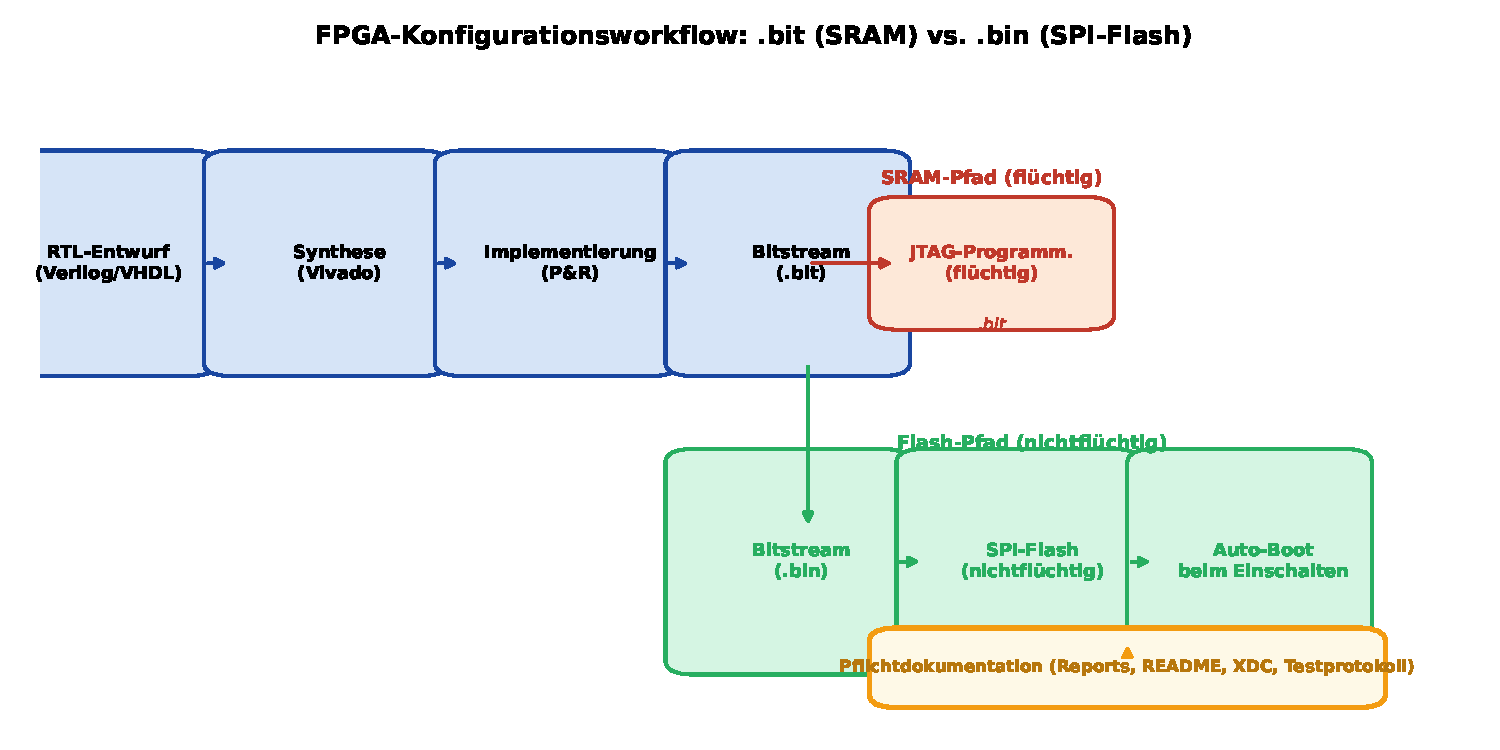
\includegraphics[width=0.95\textwidth]{plot_workflow.pdf}
    \caption{FPGA-Konfigurationsworkflow: Der \texttt{.bit}-Pfad (rot) führt
    zur flüchtigen SRAM-Konfiguration via JTAG. Der \texttt{.bin}-Pfad (grün)
    führt zur nichtflüchtigen SPI-Flash-Programmierung mit automatischem
    Boot-Verhalten. Die Dokumentationspflicht (gelb) ist an den Flash-Pfad
    gekoppelt und beginnt ab der Bitstream-Generierung.}
    \label{fig:workflow}
\end{figure}

Abbildung~\ref{fig:workflow} zeigt beide Konfigurationspfade im Vergleich.
Der wesentliche Unterschied liegt nicht in der Logikfunktion (Lemma~\ref{lem:aequiv}),
sondern in der \emph{Persistenz} und den daraus folgenden Anforderungen.

\begin{table}[htbp]
    \centering
    \caption{Vergleich der FPGA-Konfigurationsformate.}
    \label{tab:vergleich}
    \begin{tabular}{@{}lll@{}}
        \toprule
        Eigenschaft & \texttt{.bit} (SRAM) & \texttt{.bin} (Flash) \\
        \midrule
        Persistenz & Flüchtig & Nichtflüchtig ($\geq 20$ Jahre) \\
        Ladezeit & $< 1$\,s (JTAG) & $< 500$\,ms (SPI, autonom) \\
        Programmierwerkzeug & Vivado Hardware Manager & Vivado / OpenOCD \\
        Autonomes Booten & Nein & Ja \\
        Eignung Entwicklung & Sehr hoch & Mittel \\
        Eignung Produktion & Gering & Sehr hoch \\
        Dokumentationspflicht & Empfohlen & \textbf{Zwingend} \\
        ISO-26262-relevant & Nein & Ja (bei Automotive) \\
        \bottomrule
    \end{tabular}
\end{table}

\begin{figure}[htbp]
    \centering
    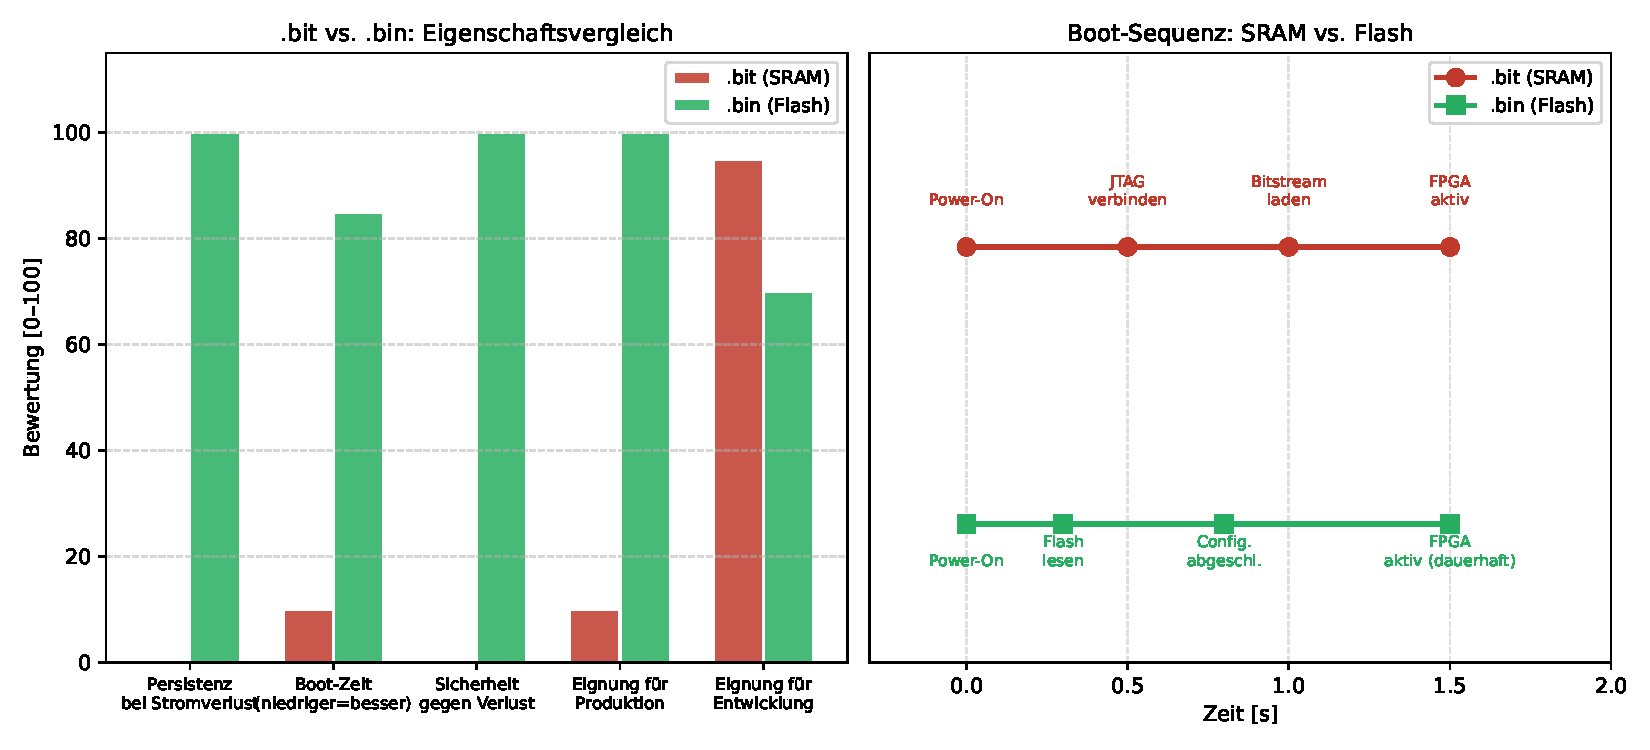
\includegraphics[width=0.92\textwidth]{plot_bitbin.pdf}
    \caption{Links: Eigenschaftsvergleich \texttt{.bit} vs. \texttt{.bin} nach
    sechs Kriterien. Persistenz und Produktionseignung sprechen klar für Flash;
    Entwicklungseignung und einfaches Nachladen für SRAM.
    Rechts: Boot-Sequenz beider Pfade im Zeitstrahl — Flash konfiguriert den
    FPGA autonom beim Einschalten ohne externe Werkzeuge.}
    \label{fig:bitbin}
\end{figure}

\subsection{Formale Eigenschaften}

\begin{satz}[Autonomie der Flash-Konfiguration]
    \label{satz:auto}
    Ein mit \texttt{.bin} programmierter FPGA konfiguriert sich nach jedem
    Power-On-Reset ohne externe Eingriffe korrekt:
    \[
    \forall t_{\rm power} > 0: f_{\kappa(\mathcal{B}_{\rm bin})}
    \text{ ist aktiv nach } t_{\rm power} + t_{\rm Flash}.
    \]
\end{satz}

\begin{proof}
    Der Artix-7 Konfigurationscontroller liest nach dem Anlegen von $V_{DD}$
    im Master-SPI-Modus den Flash-Speicher sequenziell aus. Da der Flash-Inhalt
    nichtflüchtig ist (Definition~3), ist $\mathcal{B}_{\rm bin}$ zu jedem
    Zeitpunkt $t > 0$ verfügbar. Die Konfiguration $\kappa(\mathcal{B}_{\rm bin})$
    wird deterministisch in $t_{\rm Flash} < 500$\,ms abgeschlossen.
    Nach Abschluss ist $f_c$ aktiv. Da dieser Prozess keiner externen
    Aktion bedarf, gilt die Autonomieeigenschaft für jeden Power-On-Zyklus.
    \qedhere
\end{proof}

\begin{korollar}[Gerätestatus]
    Ein FPGA mit Flash-Konfiguration ist ab dem Zeitpunkt der Programmierung
    ein eigenständiges, autonomes Hardwaregerät, das seine Funktion ohne
    Entwicklungsinfrastruktur ausführt.
\end{korollar}

% ──────────────────────────────────────────────────────────────
\section{Formale Dokumentationspflicht}
\label{sec:pflicht}

\subsection{Herleitung der Pflicht}

\begin{satz}[Dokumentationspflicht für nichtflüchtige Designs]
    \label{satz:pflicht}
    Sei $\mathcal{E}$ ein FPGA-Entwurf, der in den SPI-Flash eines Boards
    programmiert wird. Dann ist eine vollständige Dokumentation
    $\mathcal{D} = (S, X, R, T, M)$ eine notwendige Bedingung für:
    \begin{enumerate}
        \item Reproduzierbarkeit: Den Entwurf aus den Quelldateien neu erzeugen.
        \item Wartbarkeit: Den Entwurf nach der Erstellung modifizieren.
        \item Verständlichkeit: Die Funktion des Designs ohne den Entwickler erklären.
        \item Verifikation: Korrektheit des Designs nachweisen.
    \end{enumerate}
\end{satz}

\begin{proof}
    Wir beweisen jeden der vier Punkte durch Widerspruch.

    \textbf{(1) Reproduzierbarkeit.}
    Angenommen, $S = \emptyset$ (keine Quelldateien). Da der Bitstrom
    $\mathcal{B}_{\rm bin}$ im Allgemeinen nicht rückwärts in RTL-Code
    dekompilierbar ist (NP-schweres Reverse-Engineering-Problem~\cite{quadrant2020}),
    kann $\mathcal{E}$ nicht reproduziert werden. Widerspruch zur Anforderung (1).
    Also $S \neq \emptyset$.

    \textbf{(2) Wartbarkeit.}
    Angenommen, $X = \emptyset$ (keine Constraints). Eine Modifikation von
    $\mathcal{E}$ erfordert Neusynthese und Implementierung. Ohne XDC-Datei
    sind Pin-Zuordnungen unbekannt; eine falsche Pinbelegung führt zu
    Schäden an Board oder Peripherie. Also $X \neq \emptyset$.

    \textbf{(3) Verständlichkeit.}
    Angenommen, $M = \emptyset$ (keine Benutzerdokumentation). Ein autonomes
    Gerät ohne Beschreibung seiner Ein-/Ausgänge, Schalterstellungen und
    LEDs ist für jeden Nutzer außer dem Entwickler unverständlich.
    Da das Gerät autonom bootet (Satz~\ref{satz:auto}), ist keine
    Entwicklungsumgebung zur Inspektion verfügbar. Also $M \neq \emptyset$.

    \textbf{(4) Verifikation.}
    Angenommen, $T = \emptyset$ (kein Testprotokoll). Dann ist unklar, ob
    das Design korrekt ist. Bei nichtflüchtiger Programmierung ist das
    Design dauerhaft aktiv; ein unkorrekt verifiziertes Design kann
    dauerhaft Schäden erzeugen. Also $T \neq \emptyset$.

    Da alle fünf Komponenten nicht leer sein müssen, ist $\mathcal{D}$ vollständig.
    \qedhere
\end{proof}

\begin{lemma}[Zeitpunkt der Dokumentationspflicht]
    \label{lem:zeitpunkt}
    Die Dokumentationspflicht beginnt spätestens mit der Entscheidung,
    den Bitstrom in den SPI-Flash zu schreiben — nicht erst danach.
\end{lemma}

\begin{proof}
    Sei $t_F$ der Zeitpunkt der Flash-Programmierung. Nach $t_F$ ist das
    Gerät autonom (Satz~\ref{satz:auto}). Die Dokumentation muss zum
    Zeitpunkt $t_F$ vollständig sein, da:
    \begin{itemize}
        \item Berichte ($R$) nur vor $t_F$ aus Vivado exportierbar sind,
        \item Quelldateien ($S$) nach einer Modifikation nicht mehr mit
              dem Flash-Inhalt übereinstimmen könnten,
        \item das Testprotokoll ($T$) die Korrektheit \emph{vor} dem
              Deployment belegen muss.
    \end{itemize}
    Also muss $\mathcal{D}$ vollständig sein für $t \leq t_F$. \qedhere
\end{proof}

\begin{satz}[Dokumentation als Workflowbestandteil]
    \label{satz:workflow}
    Die Erstellung der Dokumentation $\mathcal{D}$ muss integraler
    Bestandteil des Entwurfsworkflows sein — nicht ein optionaler
    nachgelagerter Schritt.
\end{satz}

\begin{proof}
    Aus Lemma~\ref{lem:zeitpunkt} folgt, dass $\mathcal{D}$ vor $t_F$
    vollständig sein muss. Da Berichte ($R$) aus Vivado-Syntheseläufen
    stammen, die Teil des Workflows sind, und das Testprotokoll ($T$)
    die Simulation dokumentiert, die ebenfalls im Workflow stattfindet,
    können diese Dokumente nur \emph{innerhalb} des Workflows entstehen.
    Ein nachgelagerter Dokumentationsschritt würde erfordern, den gesamten
    Syntheseablauf zu wiederholen — was dem Workflow widerspricht.
    Also ist $\mathcal{D}$ im Workflow integriert. \qedhere
\end{proof}

% ──────────────────────────────────────────────────────────────
\section{Dokumentationsworkflow}
\label{sec:workflow}

\subsection{Vollständiger Workflow}

\begin{figure}[htbp]
    \centering
    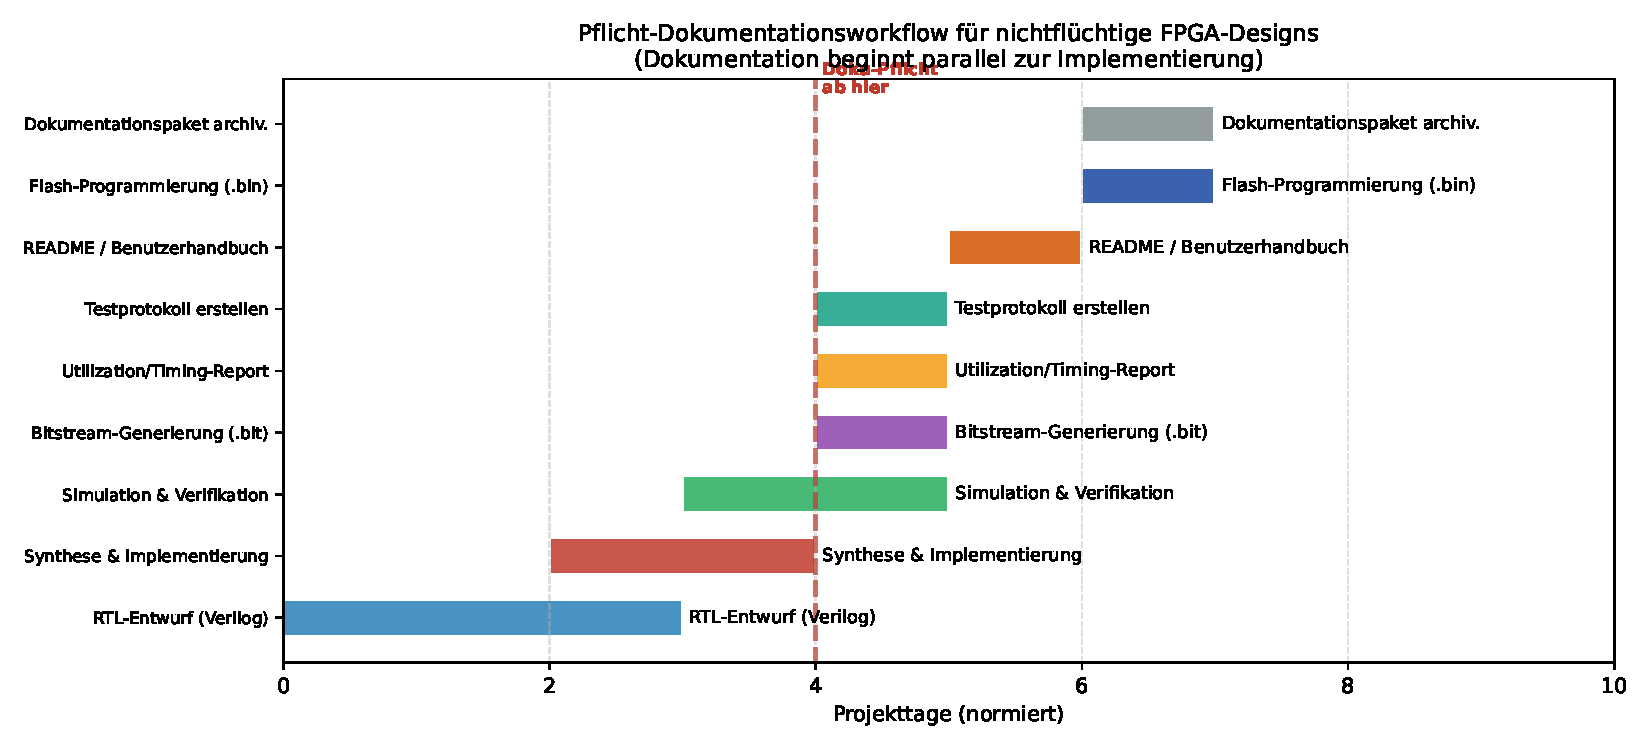
\includegraphics[width=0.92\textwidth]{plot_gantt.pdf}
    \caption{Pflicht-Dokumentationsworkflow als Gantt-Diagramm. Die rote
    gestrichelte Linie markiert den Beginn der Dokumentationspflicht
    (ab Bitstream-Generierung). Dokumentationsaufgaben laufen parallel
    zur technischen Implementierung — nicht sequenziell danach.}
    \label{fig:gantt}
\end{figure}

Abbildung~\ref{fig:gantt} zeigt den vollständigen Workflow. Der kritische
Beobachtung ist, dass Dokumentationsaufgaben ab Tag~4 (Bitstream-Generierung)
\emph{parallel} zur Implementierung laufen müssen, um Lemma~\ref{lem:zeitpunkt}
zu erfüllen.

\subsection{Dokumentationsstruktur}

\begin{figure}[htbp]
    \centering
    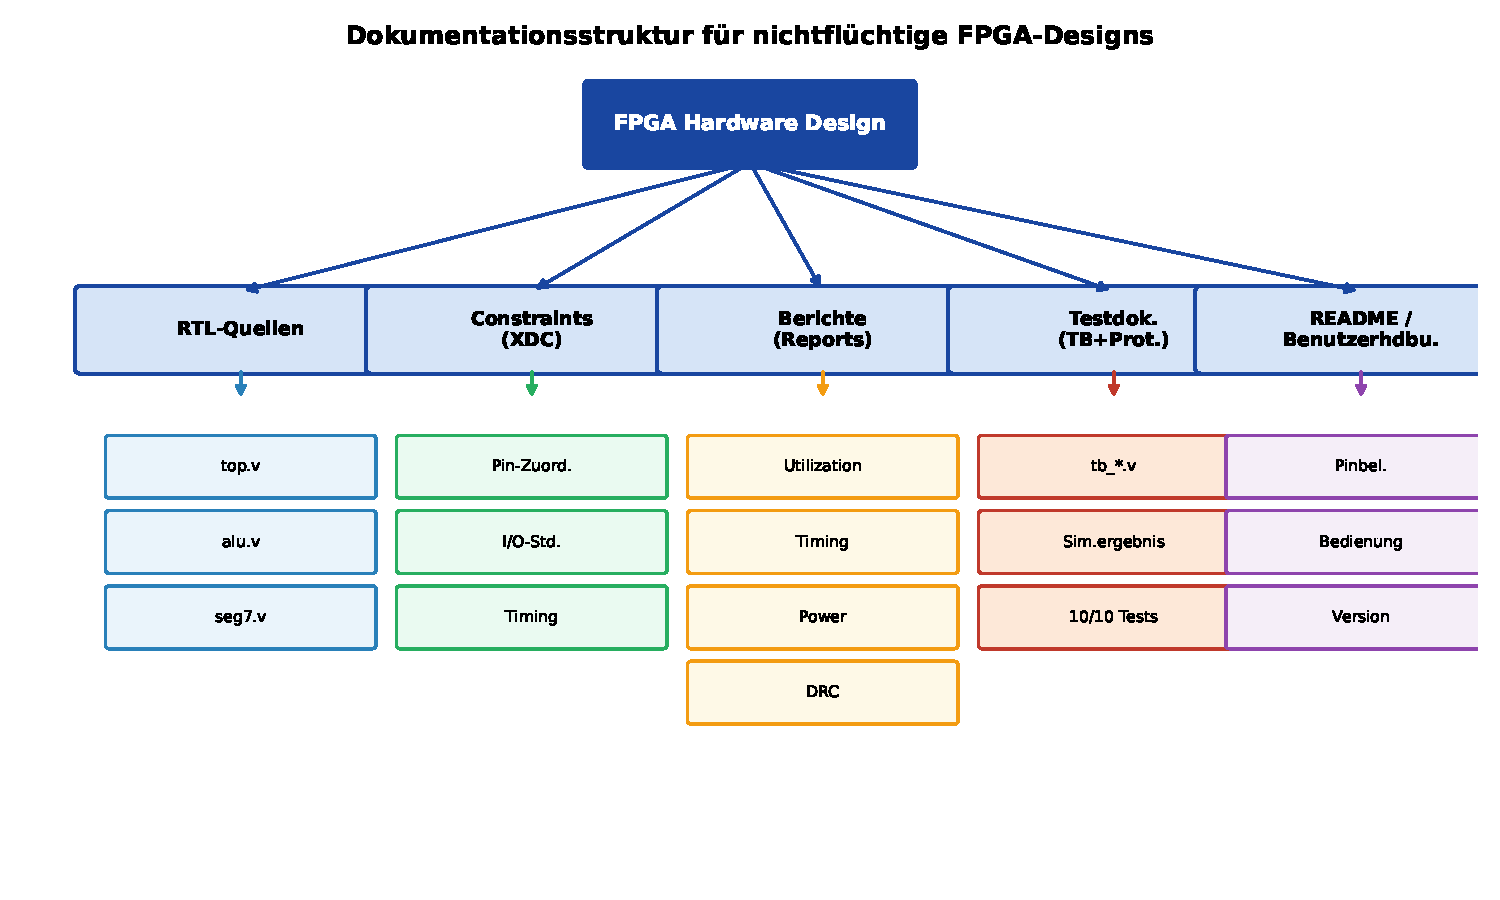
\includegraphics[width=0.92\textwidth]{plot_docstruct.pdf}
    \caption{Hierarchische Dokumentationsstruktur für FPGA-Designs.
    Fünf Hauptkategorien (RTL-Quellen, Constraints, Berichte, Testdokumentation,
    Benutzerdokumentation) mit ihren jeweiligen Artefakten. Alle fünf
    Kategorien müssen für Vollständigkeit nach Definition~5 befüllt sein.}
    \label{fig:docstruct}
\end{figure}

\begin{definition}[Pflicht-Dokumentationspaket]
    Ein Pflicht-Dokumentationspaket $\mathcal{P}$ für ein nichtflüchtiges
    FPGA-Design ist das geordnete Tupel:
    \[
    \mathcal{P} = \mathcal{D} \cup \{\mathcal{B}_{\rm bin}, v, h\},
    \]
    wobei $v$ die Versionsnummer und $h$ der SHA-256-Hash des Bitstroms sind,
    sodass Bitstrom und Dokumentation eindeutig verknüpft sind:
    \[
    h = \mathrm{SHA256}(\mathcal{B}_{\rm bin}).
    \]
\end{definition}

\begin{lemma}[Integrität des Dokumentationspakets]
    Der Hash $h = \mathrm{SHA256}(\mathcal{B}_{\rm bin})$ garantiert,
    dass Dokumentation und Bitstrom zusammengehören:
    \[
    h' = \mathrm{SHA256}(\mathcal{B}'_{\rm bin}) \neq h
    \implies \mathcal{B}'_{\rm bin} \neq \mathcal{B}_{\rm bin}.
    \]
\end{lemma}

\begin{proof}
    Direkte Folge der Kollisionsresistenz von SHA-256~\cite{nist2015}:
    Für verschiedene Bitstromversionen $\mathcal{B} \neq \mathcal{B}'$
    gilt mit kryptographischer Sicherheit $h \neq h'$. \qedhere
\end{proof}

\subsection{Vivado-Berichte als Dokumentationsartefakte}

\begin{figure}[htbp]
    \centering
    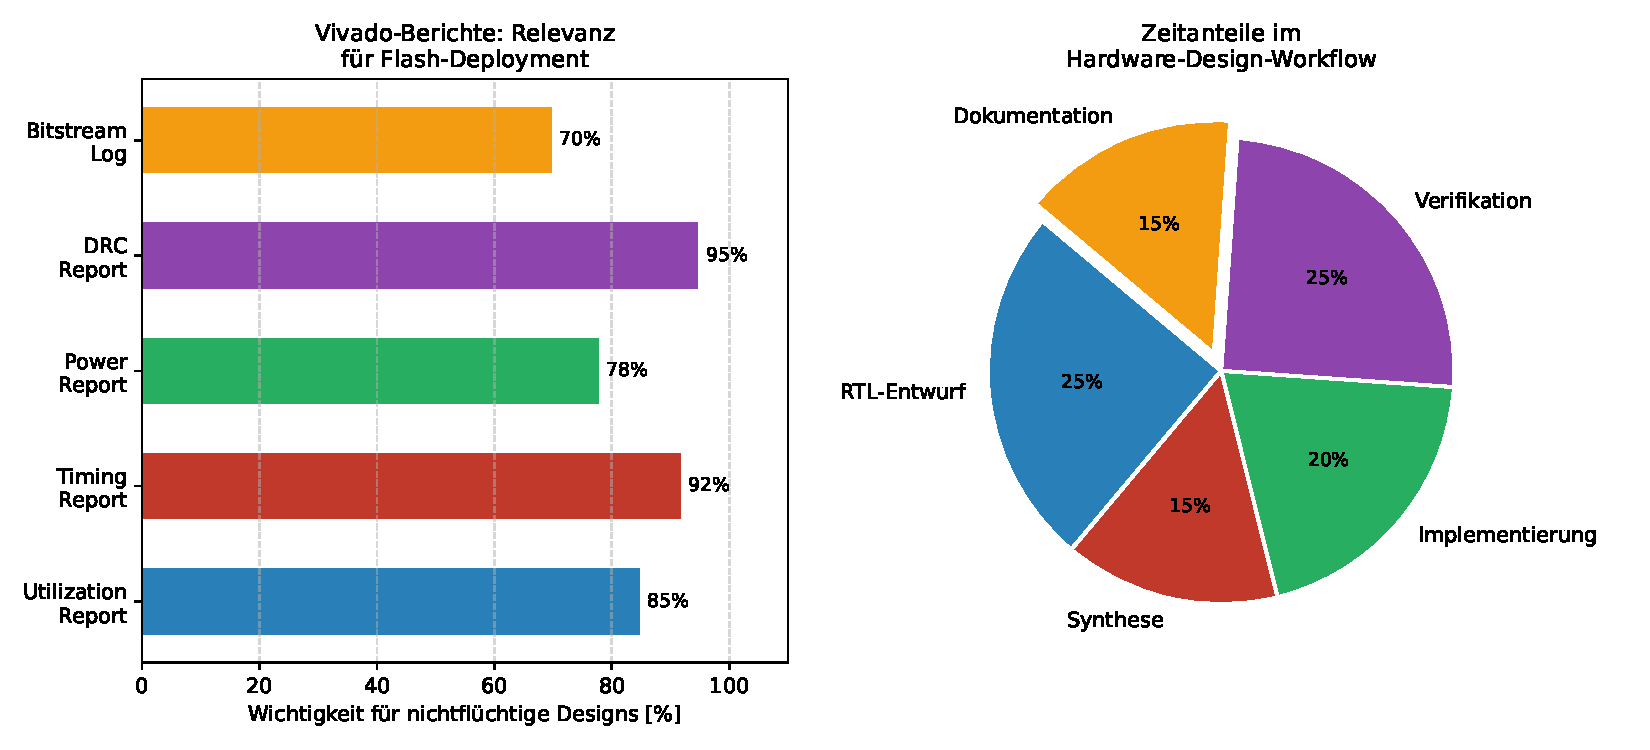
\includegraphics[width=0.92\textwidth]{plot_reports.pdf}
    \caption{Links: Relevanz der Vivado-Berichte für nichtflüchtige Designs.
    DRC- und Timing-Report sind am kritischsten, da sie Korrektheit und
    Zuverlässigkeit belegen. Rechts: Zeitanteile im Entwurfsworkflow —
    Dokumentation (15\,\%) ist gleichwertig mit Synthese (15\,\%) und
    sollte entsprechend eingeplant werden.}
    \label{fig:reports}
\end{figure}

Vivado generiert automatisch folgende Berichte, die als $R \in \mathcal{D}$
archiviert werden müssen:

\begin{itemize}
    \item \textbf{Utilization Report:} Ressourcenauslastung (LUTs, FFs,
          BRAMs, DSPs). Belegt, dass das Design in den Zielbaustein passt.
    \item \textbf{Timing Report:} Setup- und Hold-Slack aller kritischen
          Pfade. Ein negativer Slack bedeutet Timing-Verletzung und
          undefiniertes Verhalten — darf nicht in den Flash.
    \item \textbf{Power Report:} Statische und dynamische Verlustleistung.
          Relevant für thermische Auslegung und Betriebssicherheit.
    \item \textbf{DRC Report:} Design Rule Checks — Verletzungen von
          Entwurfsregeln des Herstellers. Kritische DRC-Fehler verbieten
          die Flash-Programmierung.
    \item \textbf{Bitstream-Log:} Vollständige Konfigurationsparameter,
          SHA-Prüfsummen, Zieldevice-String.
\end{itemize}

% ──────────────────────────────────────────────────────────────
\section{Anwendung auf das Basys~3 (Artix-7)}
\label{sec:basys3}

\subsection{Hardwareplattform}

Das Digilent Basys~3 Board enthält:
\begin{itemize}
    \item \textbf{FPGA:} Xilinx Artix-7 XC7A35T-1CPG236C
          (33\,280 LUTs, 41\,600 FFs, 90 DSPs, 50 BRAMs)
    \item \textbf{Flash:} Winbond W25Q128JV (128\,Mbit SPI-NOR,
          $\geq 20$ Jahre Datenhaltung, 100\,000 Schreibzyklen)
    \item \textbf{Konfigurationsschnittstelle:} JTAG (über USB-UART-Bridge)
          und Master-SPI (auto-boot aus Flash)
    \item \textbf{Programmiermodus:} Jumper JP1 wählt zwischen
          JTAG-only und Master-SPI-Flash-Boot
\end{itemize}

\subsection{Flash-Programmierung in Vivado}

Der Workflow für die \texttt{.bin}-Erzeugung in Vivado~2019.2:

\begin{enumerate}
    \item \textbf{Bitstream-Einstellungen:} In den Project Settings unter
          \texttt{Bitstream} die Option \texttt{-bin\_file yes} aktivieren.
          Vivado erzeugt dann zusätzlich zum \texttt{.bit} auch ein \texttt{.bin}.
    \item \textbf{Hardware Manager öffnen:} \texttt{Open Hardware Manager
          → Open Target → Auto Connect}.
    \item \textbf{Flash programmieren:} Rechtsklick auf den FPGA
          \texttt{→ Add Configuration Memory Device → Winbond W25Q128}
          \texttt{→ Program Configuration Memory Device → .bin auswählen}.
    \item \textbf{Jumper setzen:} JP1 auf \texttt{SPI} (nicht JTAG).
    \item \textbf{Neustart:} Stromversorgung trennen und wieder anlegen —
          der FPGA bootet autonom aus dem Flash.
\end{enumerate}

\subsection{Pflichtdokumentationspaket für das ALU-Projekt}

Als konkretes Beispiel zeigt Tabelle~\ref{tab:alupaket} das vollständige
Pflicht-Dokumentationspaket für das ALU-Projekt auf dem Basys~3.

\begin{table}[htbp]
    \centering
    \caption{Pflicht-Dokumentationspaket für das Basys~3 ALU-Projekt.}
    \label{tab:alupaket}
    \begin{tabular}{@{}lll@{}}
        \toprule
        Kategorie & Artefakt & Status \\
        \midrule
        $S$ (Quellen)      & \texttt{top.v}, \texttt{alu.v}, \texttt{seg7\_mux.v} & Vorhanden \\
        $X$ (Constraints)  & \texttt{basys3\_alu.xdc}                              & Vorhanden \\
        $R$ (Berichte)     & Utilization, Timing, Power, DRC                       & Aus Vivado \\
        $T$ (Test)         & \texttt{tb\_top.v}, Simulationsprotokoll              & Vorhanden \\
        $M$ (Benutzer)     & \texttt{README.md}, Pinbelegung, Operationstabelle    & Vorhanden \\
        $\mathcal{B}$      & \texttt{top.bin}                                      & Aus Vivado \\
        $h$                & SHA-256(\texttt{top.bin})                             & Zu erzeugen \\
        $v$                & v1.0.0 (Git-Tag)                                      & Vorhanden \\
        \bottomrule
    \end{tabular}
\end{table}

% ──────────────────────────────────────────────────────────────
\section{Zusammenfassung}

Diese Arbeit hat formal nachgewiesen, dass die nichtflüchtige Konfiguration
eines FPGA mittels SPI-Flash eine vollständige Dokumentationspflicht impliziert.

Die zentralen Ergebnisse sind:
\begin{itemize}
    \item \texttt{.bit} (SRAM) und \texttt{.bin} (Flash) implementieren
          dieselbe Logikfunktion (Lemma~\ref{lem:aequiv}), unterscheiden sich
          aber fundamental in Persistenz und Autonomieverhalten.
    \item Ein Flash-programmierter FPGA ist ein autonomes Hardwaregerät
          (Satz~\ref{satz:auto}), das ohne externe Werkzeuge bootet.
    \item Für nichtflüchtige Designs ist eine vollständige Dokumentation
          $\mathcal{D} = (S, X, R, T, M)$ notwendig (Satz~\ref{satz:pflicht}).
    \item Die Dokumentation muss vor dem Flash-Deployment vollständig sein
          (Lemma~\ref{lem:zeitpunkt}).
    \item Dokumentation ist integraler Workflowbestandteil, kein nachgelagerter
          Schritt (Satz~\ref{satz:workflow}).
    \item SHA-256-Hashing verknüpft Bitstrom und Dokumentation
          fälschungssicher (Lemma~5).
    \item Vivado-Berichte (Utilization, Timing, Power, DRC) sind
          Pflichtartefakte der Dokumentationskomponente~$R$.
\end{itemize}

% ──────────────────────────────────────────────────────────────
\section{Ausblick}
\label{sec:ausblick}

\subsection{Automatisierte Dokumentationsgenerierung in Vivado}

Der in dieser Arbeit spezifizierte Dokumentationsworkflow lässt sich in Vivado
vollständig automatisieren. Vivado stellt eine TCL-Skriptschnittstelle zur
Verfügung, über die alle Berichte, Bitstreams und Metadaten programmatisch
erzeugt werden können. Ein vollständiges TCL-Skript könnte nach jedem
erfolgreichen Implementierungslauf automatisch ausgeführt werden:

\begin{lstlisting}[language=tcl, caption={Automatisiertes Dokumentations-TCL-Skript}]
# Nach Generate Bitstream ausfuehren
open_run impl_1
report_utilization -file docs/utilization.rpt
report_timing_summary -file docs/timing.rpt
report_power -file docs/power.rpt
report_drc -file docs/drc.rpt
write_bitstream -bin_file -force output/top.bin
# SHA-256 Hash berechnen
exec sha256sum output/top.bin > docs/top.bin.sha256
\end{lstlisting}

Dieses Skript könnte als \emph{Post-Implementation Hook} in den Vivado-Flow
integriert werden: \texttt{Tools → Settings → Implementation → Tcl Scripts
→ tcl.post}. Damit ist sichergestellt, dass kein Bitstrom ohne vollständige
Dokumentation erzeugt werden kann — die Pflicht wird technisch durchgesetzt.

\subsection{Versionskontrolle und Dokumentation}

Die Integration von Git als Versionskontrollsystem in den FPGA-Entwurfsworkflow
ist eine natürliche Erweiterung. Jeder Commit, der eine neue \texttt{.bin}-Version
erzeugt, sollte automatisch folgende Dateien enthalten:
\begin{itemize}
    \item Alle RTL-Quelldateien ($S$)
    \item Constraints ($X$)
    \item Generierte Berichte ($R$) als Textdateien
    \item Testbench-Ergebnisse ($T$)
    \item Aktualisierte README ($M$)
    \item Den SHA-256-Hash des Bitstroms (nicht den Bitstrom selbst —
          Binärdateien in Git sind ungünstig für Diffs)
\end{itemize}

Git-Tags (z.\,B. \texttt{v1.0.0}, \texttt{v2.0.0}) markieren
Release-Stände, die einem programmierten Flash-Inhalt entsprechen.
Damit ist zu jedem Zeitpunkt rekonstruierbar, welcher Quellcode zu
welchem Flash-Inhalt gehört.

\subsection{Formale Verifikation des Designs als Dokumentationsbestandteil}

Ein wichtiger zukünftiger Schritt ist die Integration formaler
Verifikationsmethoden in den Dokumentationsworkflow. Formale Methoden
liefern maschinengeprüfte Korrektheitsnachweise — stärker als
simulationsbasierte Tests, die nur endlich viele Testfälle abdecken.

Für FPGA-Designs bieten sich folgende Ansätze an:
\begin{itemize}
    \item \textbf{Symbio\-lische Simulation:} Tools wie SymbiYosys
          (Open-Source, basierend auf Yosys + Z3) ermöglichen die formale
          Verifikation von Verilog-Designs durch Bounded Model Checking.
          Ein Beweis der Form ``Die ALU liefert für alle Eingaben das
          korrekte Ergebnis'' ist damit maschinengeprüft.
    \item \textbf{Formale Äquivalenzprüfung:} Yosys \texttt{equiv\_check}
          vergleicht RTL und Post-Synthese-Netlist formell auf Äquivalenz.
          Dies stellt sicher, dass der Syntheseprozess keine Logikfehler
          einführt.
    \item \textbf{Property Checking:} SystemVerilog Assertions (SVA) können
          in Vivado-Simulationen und formalen Tools genutzt werden, um
          Invarianten des Designs zu spezifizieren und zu beweisen.
\end{itemize}

Die Ergebnisse dieser formalen Verifikation sollten als eigene Komponente
$V$ in die Dokumentation aufgenommen werden:
$\mathcal{D}^+ = (S, X, R, T, M, V)$.

\subsection{Dokumentationsstandards: ISO~26262 und IEC~62304}

Für sicherheitskritische Anwendungen von FPGA-Designs — Automotive, Medizintechnik,
Industrieautomation — schreiben Normen die Dokumentation zwingend vor.

ISO~26262 (Funktionale Sicherheit für Straßenfahrzeuge) fordert für
Hardware-Entwicklung auf ASIL-B und höher:
\begin{itemize}
    \item Hardware-Sicherheitsanforderungsspezifikation (HSRS)
    \item Hardware-Entwurfsbeschreibung (inkl. Block-Diagramme, Schnittstellen)
    \item Hardware-Integrations- und -Verifikationsplan (HIVP)
    \item Hardware-Qualifizierungstest (HQT)
\end{itemize}

Alle diese Dokumente entsprechen den in dieser Arbeit definierten Komponenten
$(S, X, R, T, M)$ und bestätigen die Allgemeingültigkeit des formalen
Dokumentationsrahmens.

\subsection{Digitaler Zwilling und Dokumentation}

Das Konzept des \emph{Digitalen Zwillings} — ein virtuelles Modell eines
physikalischen Geräts, das synchron mit dem realen Gerät gehalten wird —
ist eine natürliche Erweiterung des Dokumentationspakets
$\mathcal{P}$. Für ein Flash-programmiertes FPGA-Board wäre der
digitale Zwilling:
\begin{itemize}
    \item Das vollständige RTL-Modell (simulierbar in Vivado / Icarus Verilog)
    \item Der verifizierte Bitstrom mit SHA-256-Hash
    \item Die Timing-Charakteristik des konkreten Bausteins
    \item Ein Zustandsmodell der externen Schnittstellen (LEDs, Schalter, GPIO)
\end{itemize}

Dieser Zwilling erlaubt es, das Verhalten des physikalischen Boards vollständig
in Software zu simulieren — für Regressionstests, Fehleranalyse und
Weiterentwicklung ohne das physikalische Board.

\subsection{Blockchain-basierte Dokumentationsintegrität}

Für höchste Anforderungen an die Unveränderlichkeit der Dokumentation —
etwa in der Medizintechnik oder Luft- und Raumfahrt — bietet sich die
Speicherung des Dokumentations-Hashes auf einer öffentlichen oder
permissioned Blockchain an. Damit ist:
\begin{itemize}
    \item Die Existenz der Dokumentation zum Zeitpunkt $t_F$ beweisbar
    \item Jede nachträgliche Änderung nachweisbar (Audit Trail)
    \item Die Verknüpfung von Bitstrom $h = \mathrm{SHA256}(\mathcal{B}_{\rm bin})$
          und Dokumentation unveränderlich
\end{itemize}

Der Ethereum-Blockchain-Smart-Contract könnte in Solidity implementiert werden
und eine Funktion \texttt{registerDesign(bytes32 bitstromHash, bytes32 docHash)}
bereitstellen.

\subsection{Open-Source-Toolchain: fpgadoc}

Aus den Erkenntnissen dieser Arbeit lässt sich eine Open-Source-Toolchain
\texttt{fpgadoc} ableiten, die folgende Komponenten integriert:

\begin{enumerate}
    \item \textbf{Report-Parser:} Liest Vivado-XML-Reports und extrahiert
          Schlüsselkennzahlen (Slack, LUT-Auslastung, Leistung).
    \item \textbf{README-Generator:} Erzeugt automatisch eine strukturierte
          README aus den Report-Daten und der XDC-Datei.
    \item \textbf{Hash-Manager:} Berechnet SHA-256 des \texttt{.bin}-Files
          und verknüpft ihn mit dem Git-Commit.
    \item \textbf{Vollständigkeitsprüfer:} Prüft, ob alle Komponenten
          von $\mathcal{D}$ vorhanden sind, bevor die Flash-Programmierung
          freigegeben wird.
    \item \textbf{Archivierungs-Pipeline:} Packt das vollständige
          $\mathcal{P}$ als versioniertes ZIP-Archiv.
    \item \textbf{CI/CD-Integration:} GitHub Actions / GitLab CI-Skripte,
          die den gesamten Workflow von RTL-Commit bis zum archivierten
          Dokumentationspaket automatisieren.
\end{enumerate}

Eine solche Toolchain würde den in Satz~\ref{satz:workflow} bewiesenen
Grundsatz — Dokumentation als integraler Workflowbestandteil — technisch
erzwingen.

\subsection{Verbindung zum Subgraph Algorithmus}

Der Subgraph Algorithmus~\cite{epp2026} bietet eine interessante Perspektive
für die Dokumentationsintegrität: Zwei Versionen eines FPGA-Designs können
als Graphen dargestellt werden (Knoten = Logikblöcke, Kanten = Verbindungen).
Der Subgraph-Vergleich zweier Versionen identifiziert strukturelle Änderungen
und kann automatisch prüfen, ob die Dokumentation entsprechend aktualisiert wurde:
\begin{itemize}
    \item Neue Kanten im Designgraph → neue Verbindungen → XDC muss
          aktualisiert sein.
    \item Neue Knoten → neue Logikblöcke → Utilization-Report muss
          sich geändert haben.
    \item Identische Graphen bei verschiedenen Versionsnummern → Warnung:
          möglicherweise unnötiger Release.
\end{itemize}

% ──────────────────────────────────────────────────────────────
\begin{thebibliography}{99}

\bibitem{xilinx2019}
Xilinx Inc.,
\emph{Vivado Design Suite User Guide: Programming and Debugging (UG908)},
Version 2019.2, Xilinx, 2019.

\bibitem{digilent2023}
Digilent Inc.,
\emph{Basys~3 Reference Manual},
Revision C, Digilent, 2023.
\url{https://digilent.com/reference/programmable-logic/basys-3/reference-manual}

\bibitem{winbond2021}
Winbond Electronics Corp.,
\emph{W25Q128JV: 128M-Bit Serial Flash Memory with Uniform 4KB Sectors},
Datasheet Rev. M, 2021.

\bibitem{iso26262}
International Organization for Standardization,
\emph{ISO~26262: Road Vehicles — Functional Safety},
2nd Edition, ISO, 2018.

\bibitem{iec62304}
International Electrotechnical Commission,
\emph{IEC~62304: Medical Device Software — Software Life Cycle Processes},
Edition 1.1, IEC, 2015.

\bibitem{quadrant2020}
C. Wolf,
\emph{Yosys Open SYnthesis Suite — Internals and Applications},
Proceedings of the Free and Open Source Silicon Foundation, 2020.
\url{https://yosyshq.net}

\bibitem{nist2015}
National Institute of Standards and Technology,
\emph{FIPS PUB 180-4: Secure Hash Standard (SHS)},
NIST, 2015.

\bibitem{symbiyosys}
C. Wolf und N. Ecki,
\emph{SymbiYosys: Formal Hardware Verification Front-End for Yosys},
Open-Source Tool, 2022.
\url{https://symbiyosys.readthedocs.io}

\bibitem{epp2026}
S. Epp,
\emph{Der Subgraph Algorithmus},
Technischer Bericht, 2026.
\url{https://gitlab.com/epp-group/subgraph}

\end{thebibliography}

\end{document}

